\subsubsection{Generic distributed system frameworks}
Distributed system already exist for companies possessing massive amounts of data that they want to be able to query and analyze. These frameworks largely rely on multiple commodity servers, each of them with a relatively small storage capacity and computing power, rather than one expensive large server. This strategy has proven more affordable, as long as sufficient fault tolerance is built into the software.

\paragraph{The frameworks}
The storage layer of existing frameworks is commonly based on the \textit{Google File System (GFS)}\cite{Ghem03}. GFS is owned by and used within Google to handle all Big Data storage needs within the company. GFS splits the data that is uploaded to the cluster up into chunks, which are then distributed over the "chunk servers" in the node. The chunks are replicated a predefined number of times (usually 3) in order to protect against data loss on server failure. The data on the chunk servers can then be accessed by a user through contacting the master, which knows exactly on which servers each chunk is stored.\cite{Ghem03} The data and work-flow is described in Figure \ref{GFS_Architecture} below.

\begin{figure}
	\begin{center}
	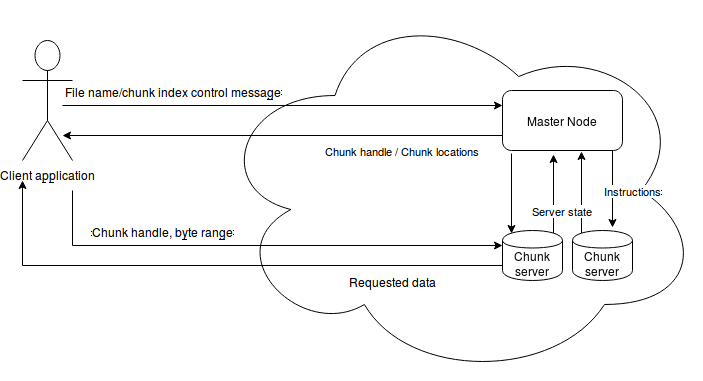
\includegraphics[width=0.8\textwidth]{GFS.png}
	\caption{Google File System architecture}%\cite{Ghem03}
	\label{GFS_Architecture}
	\end{center}
\end{figure}

The GFS architecture as first described by \citep{Ghem03} was adopted by an open-source framework called Hadoop \cite{Shv10}. Hadoop was developed mainly by Yahoo!, and is now distributed and maintained as an Apache project. Its storage layer, named Hadoop File System or HDFS, functions essentially the same as GFS. There are only minor differences with GFS, such as the naming of certain subsystems and the chunk size. A typical use case of adding a file to the Hadoop File System (HDFS) is show in Figure \ref{Hadoop_usecase} below. \ref{Hadoop_usecase} below.

\begin{figure}
	\begin{center}
	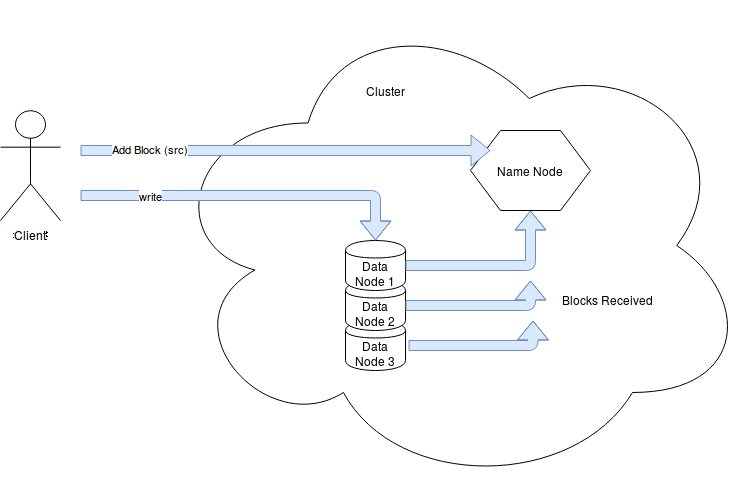
\includegraphics[width=0.8\textwidth]{HDFS.png}
	\caption{The data flow when adding a file to the HDFS}%\cite{Shv10}
	\label{Hadoop_usecase}
	\end{center}
\end{figure}

\paragraph{Uses of the frameworks}
The storage architecture highlighted above is the most common one empowering Big Data frameworks today. Popular examples of these are MapReduce and the Apache Spark engine.

\paragraph{MapReduce}
MapReduce is a framework (and underlying architecture) for processing data, and was developed by Google\cite{Dean04} in order to process data in a distributed setting. The architecture consists of multiple phases. First, all data is split into tuples (called key-value pairs) during the \textit{map phase}. Then, during the \textit{shuffle phase}, these tuples are shuffled and passed on. In the \textit{reduce phase} that comes after, a calculation (often an aggregation) is performed on the tuples to generate a single output value per key. The main benefit of this framework is that the data can be distributed across a large number of machines. Those same machines can be nodes in a GFS (or similar) storage cluster, so that instead of moving data to the program, the program can be moved to the data. The program is usually several orders of magnitude smaller. It is therefore much more efficient to pass around. %TODO: A general overview of the execution of a MapReduce task is given in Figure \ref{mapreduce_execution}.

The MapReduce architecture is similar to the \textit{Bulk-Synchronous processing (BSP)} paradigm, which is a little older. However, there are some differences. An example of one is that the MapReduce framework does not allow communication between worker nodes in the map phase. Instead, it only allows cross-communication during the shuffle phase, in between the map and reduce phases\cite{Pace12}.\\
Since BSP and MapReduce are so similar, people have worked on transforming BSP tasks into MapReduce tasks. Goodrich et al.\cite{Goo11} has shown that all BSP programs can be converted into MapReduce programs. Other researchers have even gone as far as to say that all such tasks should be modeled as BSP tasks. They can then be run as a MapReduce task if so desired. The similarity would allow for this, and the theoretical correctness of the BSP paradigm could then leverage the efficiency of MapReduce\cite{Pace12}.

MapReduce as a framework is proprietary to Google. The architecture behind it, however, has been recreated in the aforementioned open source Hadoop framework. It leverages HDFS where MapReduce uses GFS, but is otherwise very similar.

\paragraph{Apache Spark}
Like MapReduce, Apache Spark is a service built on top of distributed file systems that can run programs in a distributed manner. It is open source, and capable of executing a directed acyclic graph of transformations (like mappings) and actions (like reductions) fully in memory\cite{Sparkwebsite}. This in contrast to MapReduce, which forces the programmer to first use a map phase and then a reduce phase. Because of its structure, Spark can be significantly faster than MapReduce. When e.g. two consecutive map phases are needed, two MapReduce tasks would need to be executed, both of which would need to write all (intermediate) data to disk. Spark, on the other hand, can keep all the data in memory, which saves expensive writes to the disk. However, it does need to take additional steps to prevent losing processed data in case of a power outage.\\

The data structure with which Spark solves this problem is called a \textit{Resilient Distributed Dataset (RDD)}. Such datasets are read-only, and new ones can only be created from data stored on the disk or by transforming existing RDDs\cite{Zaha12}. The "Resilient" part comes into play when the data is lost: each RDD is given a lineage graph that shows what transformations have been executed on it. This lineage graph ensures that, if some data is lost, Spark can trace the path the RDD has followed from the lineage graph and recalculate any lost data. It is important that the lineage graph does not contain cycles (i.e. is a Directed Acylic Graph). Otherwise Spark would run into infinite loops and be unable to recreate the RDD.
